\section{Géométrie des polyèdres}

Un \emph{polyèdre} est un sous-ensemble de $\R^n$ qui peut être écrit comme ${\mathcal P}=\{x \in \R^n |\;  Ax \geq b \}$. Un polyédre est une
intersection d'un nombre fini d'ensembles convexes et c'est donc un ensemble convexe. Soit
$\mathcal P$ un poly\`edre de
$\R^n$. La solution
$\xopt
\in \R^n$ est une
\emph{solution admissible de base}  de
$\mathcal P$ (pour les poly\`edres, \emph{sommet}, \emph{point extrême} et \emph{solution admissible de base} sont synonymes)
si  $\xopt$ est une solution admissible ($\xopt
\in {\mathcal{P}}$) et s'il y a
$n$ contraintes linéairement indépendantes actives en
$\xopt$. Une solution admissible de base $\xopt$ est \emph{dégénérée}     s'il y a plus de $n$ contraintes actives en
$\xopt$. Deux solutions admissibles de base sont \emph{adjacentes}   si elles partagent $n-1$ contraintes linéairement indépendantes
actives.\\


\newpage



\begin{enumerate}




  \item Soit le poly\`edre défini par les inégalités linéaires

    $
    \begin{array}{rcr}
      x_1+4 x_2-2x_3 & = & 7\\
      2x_2 -3x_3 & \leq & 1\\
      x_2 & \geq & 2\\
      x_3& \geq & 0
    \end{array}
    $

    Le point $(1, 2, 1)$ est-il un sommet du poly\`edre? et le point $(5, 1/2, 0)$?


    \begin{solution}
      $x = (1,2,1)$ est un sommet parce qu'il y a $n = 3$ contraintes linéairement indépendantes serrées et $x \in P$. $x = (5,\frac{1}{2},0)$ n'est pas un sommet parce que $x \not\in P$.
    \end{solution}


  \item Trouvez les sommets du poly\`edre

    $
    \begin{array}{rcr}
      -2x_1+x_2 & \leq & 2\\
      -x_1+x_2  & \leq & 3\\
      x_1 & \leq & 3\\
      x_1, x_2 & \geq & 0
    \end{array}
    $


    \begin{solution}
      Pour que $x$ soit un sommet, il faut que : \\
      - $x \in P$\\
      - $n$ contraintes linéairement indépendantes soient serrées en $x$ \\
      \newline
      Sommet : $\lbrace(1,4), (3,6), (0,2), (3,0), (0,0)\rbrace$
    \end{solution}

  \item Soit le poly\`edre défini par les inégalités linéaires

    $
    \begin{array}{rcr}
      x_1+x_2+2x_3 & \leq & 8\\
      x_2 + 6x_3 & \leq & 12\\
      x_1 & \leq & 4\\
      x_2 & \leq & 6\\
      x_1, x_2, x_3 & \geq & 0
    \end{array}
    $

    Parmi les points suivants trouvez ceux qui sont des sommets et déterminez ceux qui sont
    dégénérés: $(2, 6, 0)$, $(4, 6, 0)$, $(4, 0, 2)$. Ces sommets sont-ils adjacents?





    \begin{solution}
      - $x_{1} = (2,6,0) $ est un sommet.\\
      - $x_{2} = (4,6,0) $ n'est pas un sommet parce qu'il n'appartient pas au polyèdre.\\
      - $x_{3} = (4,0,2) $ est un sommet dégénéré. \\
      - $x_{1}$ et  $x_{3}$ ne sont pas adjacents car ils n'ont pas $n-1$ contraintes serrées communes.
    \end{solution}

  \item Trouvez  tous les sommets du poly\`edre sous forme standard ${\mathcal{P}}=\{x \in \R^4 \; | \; Ax=b \; , \; x \geq 0\}$ avec

    $
    A=
    \left[ \begin{array}{rrrr}
        1 & 0 & 2 & 0\\
        0 & 1 & -1 & -1
      \end{array}
    \right]
    \qquad
    b=
    \left[ \begin{array}{r}
        1 \\
        0
      \end{array}
    \right]$


    Déterminez les sommets adjacents et les sommets dégénérés.





    \begin{solution}
      Si $B^{-1}b \geq 0$, alors la solution est un sommet. Si une des variables de base est nulle, alors le sommet est dégénéré. \\
      $x_{1} = (1,0,0,0)$ est un sommet dégénéré. \\
      $x_{2} = (0,\frac{1}{2},\frac{1}{2},0)$ est un sommet. \\
      $x_{3} = (0,0,\frac{1}{2},-\frac{1}{2})$ n'est pas admissible car une variable de base n'est pas positive. \\
    \end{solution}

  \item Quand un demi-espace contient-il un autre demi-espace? Donnez des
    conditions pour lesquelles
    $$\{x | a^Tx \leq b \} \subseteq \{x | \tilde a ^Tx \leq \tilde b \}$$




    \begin{solution}
      Il faut que : \\
      - $a^{T} = a^{T*}$ \\
      - $ b \le b^{*}$ \\
    \end{solution}

  \item Parmi les ensembles suivants quels sont ceux qui sont des poly\`edres?

    \begin{enumerate}

      \item $\{y_1 a_1 + y_2 a_2 \; | \; -1 \leq y_1 \leq 1, \; -1 \leq y_2 \leq 1 \}$ pour des $a_1, a_2$
        donnés.

      \item $\{x \in \R^n \; | \; x \geq 0, x^T y \leq 1 \mbox{ pour tous les } y \mbox{ avec } \| y \| =1 \}$.

      \item $\{x \in \R^n \; | \; x \geq 0, x^T y \leq 1 \mbox{ pour tous les } y \mbox{ avec } \sum_i |y_i | =1 \}$.

    \end{enumerate}

    Lorsque c'est possible, exprimez l'ensemble sous forme $\{x \; | \; Ax \leq b\}$.



    \begin{solution}
      a) Oui, b) Non (Le domaine est une courbe), c) Oui \\
    \end{solution}

  \item Supposons que $\{ x \in \R^n \; | \; a_i^Tx \geq b_i, i=1, \ldots, m \}$ et $\{ x \in \R^n \; | \; g_i^Tx \geq h_i,
    i=1, \ldots, k \}$ sont deux représentation du même poly\`edre. Démontrez que si les vecteurs $a_1, \ldots, a_m$ génèrent
    $\R^n$ alors les vecteurs $g_1, \ldots, g_k$ également.







    \begin{solution}
      Un même polyèdre peut être obtenu au moyen de représentations différentes. Si le polyèdre est identique, cela signifie qu'un des deux ensembles à des contraintes linéairement dépendantes des contraintes de l'autre ensemble. \\
      \newline
      Preuve : \\
      Soient $A \in \mathbb{R}^{m \times n} $ et $B \in \mathbb{R}^{k \times n} $ des matrices telles que $Ax \geq b$ et $Bx \geq b$ représentent le même polyèdre. Supposons que $ k > m$ et que les lignes de $B$, à savoir, la suite $g_{1}, \dots, g_{k}$ n'engendrent pas $\mathbb{R}^{n}$. \\
      Dès lors, $\exists x \in \mathbb{R}^{n}$ tel que $x \notin L(B)$. Or, deux ensembles qui représentent un même polyèdre doivent avoir des contraintes communes. Il y a donc contradiction puisque, par hypothèse, l'espace ligne de $A$ forme une suite génératrice et $ k > m$. Le nombre de lignes de $B$ est donc supérieur au nombre de ligne de $A$ et les lignes de $B$ sont linéairement dépendantes des lignes de $A$. La suite $g_{1}, \dots, g_{k}$ doit donc être génératrice. %Supposons que les contraintes du domaine $Ax \geq b$ génèrent $\mathbb{R}^{n}$. Dans ce cas,
    \end{solution}

  \item Trouvez, si possible, un problème d'optimisation linéaire qui possède un coût optimal fini mais qui ne possède pas de sommet optimal.
    Trouvez, si possible, un problème  sous forme standard avec deux variables qui possède cette propriété.  Justifiez votre réponse en cas
    d'impossibilité.







    \begin{solution}
      $$\min ~x_{1}$$
      sous la contrainte : \\
      $$ x_{2} \geq 1 $$
      $$x_{1} \geq 0 $$
      Toutefois, il est impossible de trouver une solution sans sommet avec un coût fini dans le cas standard (théorème fondamental).
    \end{solution}

  \item     Considérez le problème d'optimisation

    $
    \begin{array}{lrcr}
      \mini & c^T x \\
      & Ax & \geq & b
    \end{array}
    $

    Supposez que le poly\`edre $\{x |  Ax \geq b \}$  possède au moins un sommet et que le coût optimal est fini. Vous disposez d'une routine pour résoudre les
    systèmes linéaires de $n$ équations à $n$ inconnues. La routine prévient si le déterminant est nul et retourne une solution s'il ne l'est pas. La routine
    utilise
    $O(n^3)$ opérations arithmétiques.  Proposez un algorithme
    simple de résolution du problème d'optimisation qui ne fait appel qu'à la routine. Estimez le nombre d'opérations à effectuer pour résoudre un
    problème de
    $n$ variables et $m$ contraintes. (Remarque. On écrit $f(n)=O(g(n))$ s'il existe des nombres positifs $n_0$ et $c$ pour lesquels $f(n) \leq cg(n)$ pour tout
    $n \geq n_0$.)








    \begin{solution}
      Néant
    \end{solution}

  \item Nous considérons l'ensemble $P=\{ x \in \R^n \; | \; a_i^T x \leq b_i \; , \;  i=1, \ldots, m \}$. Nous désirons trouver la
    plus grande boule entièrement contenue dans cet ensemble. Le centre de cette boule est  le {\it centre de Chebychev} de $P$.  Formulez
    ce problème comme un problème d'optimisation linéaire. Le centre de Chebychev
    existe-t-il toujours? Est-il toujours unique? (Indication:  La distance entre l'hyperplan $\{x \in \R^n | \;  a^Tx=b \}$ et le point $x_0 \in \R^n$
    est donnée par
    $|a^Tx_0 - b|/\|a\|$ avec $\|a\|=\sqrt{a_1^2+ \ldots + a_n^2}$.)



    \begin{solution}
      Le centre de Chebychev n'existe pas toujours. Ex : le domaine est non-borné. Le centre de Chebychev n'est pas toujours unique. Ex : un domaine en forme de rectangle.
    \end{solution}

  \item  Le poly\`edre de $\R^3$ défini par les inégalités linéaires

    $
    \begin{array}{rcr}
      4x_1- x_2 +x_3 & \leq & 7\\
      -x_1 +3x_2 -x_3 & \leq & 9\\
      -x_1 + 6 x_2 +5 x_3 & \leq & 5\\
      x_1, x_2, x_3 & \geq & 0
    \end{array}
    $

    est borné, possède un sommet et contient une sphère de rayon strictement positif. Nous désirons trouver le rayon de la plus grande
    sphère entièrement contenue dans ce poly\`edre. Formulez ce problème comme un problème d'optimisation et transformez le en un
    problème d'optimisation linéaire.  Répondez à la question suivante sans faire aucun calcul. Parmi les sphères de rayon
    maximum, en existe-t-il une qui touche quatre des plans qui définissent le poly\`edre? Justifiez votre réponse.






    \begin{solution}
      Néant
    \end{solution}

  \item Nous considérons un ensemble de $m$ lampes situées dans le  plan et éclairant $n$
    tronçons (voir figure).  Les variables du problèmes sont les puissances des lampes $p_1, \ldots, p_m$ qui peuvent varier entre 0 et 1 ($0 \leq p_j \leq 1$ pour
    $j=1, \ldots, m$).  L'illumination $I_i$ du point milieu du tronçon $i$ dépend de la position des lampes et de leurs
    puissances. Nous utilisons un modèle simple d'illumination

    $$I_i = \sum_{j=1}^m a_{ij} p_j$$

    où les $a_{ij}$ sont donnés. Le problème consiste à déterminer la puissance des lampes de façon à ce que les niveaux d'illumination des
    tronçons soient tous proches du niveau désiré $I_{des}$. Nous choisissons la déviation maximum

    $$\max_{i=1, \ldots, n} | I_i -I_{des}|$$

    pour quantifier la déviation globale par rapport au niveau d'illumination désiré.  Formulez ce problème comme un problème d'optimisation linéaire. Supposons
    que pour une configuration donnée de 5 lampes et 8 tronçons la déviation maximum optimale  $I^*$ est obtenue pour des puissances de lampes {\it
    strictement}  comprises entre 0 et 1 ($0 < p_j < 1$ pour $j=1, \ldots, m$). Pour combien de tronçons la déviation maximum optimale $I^*$ est-elle atteinte?





    \begin{solution}
      Néant
    \end{solution}

  \item On dispose des points $(x_i, y_i)$ expérimentaux suivants: $(0, 0), (1, 3), (2, 4)$ et $(4, 2)$. On cherche l'équation de la
    droite $y=ax+b$ qui minimise la mesure d'erreur

    $$\max_i | (ax_i+b)-y_i |.$$

    Formulez ce problème comme un problème d'optimisation linéaire. Soit
    $$z_* = \min_{a, b} \max_i|(ax_i+b)-y_i|,$$ pour combien de points
    $(x_i, y_i)$ l'égalité
    $z_*= | (ax_i+b)-y_i |$ est-elle obtenue? Considérons la généralisation de ce problème à $m$ points $(x_i, y_i)$ et à un polynôme $p(x)$ de degré $n$. On
    cherche à minimiser la mesure d'erreur

    $$\max_i | p(x_i)-y_i |.$$

    Soit $z_*$ l'objectif optimal de ce problème. Discutez le nombre de points $(x_i, y_i)$ pour lesquels $z_*= | p(x_i)-y_i|$. Supposons que ce problème
    possède plusieurs solutions. Parmi l'ensemble des solutions du problème nous cherchons celle pour laquelle la quantité

    $$\sum_i | (ax_i+b)-y_i |$$

    est minimum. Comment formuler ce problème comme un problème d'optimisation linéaire?




    \begin{solution}
      $$\min ~t$$
      $$ -t \le ax_{i} + b - y_{i} \le t $$
      L'erreur sera nulle pour au moins deux points. \\
      $$\min \sum_{i}^{n} t_{i}$$
      $$-t_{i} \le ax_{i} + b - y_{i} \le t_{i}$$
    \end{solution}

  \item  Soit $\| \cdot \|_{\infty}$ la norme du maximum ($\| x \|_{\infty}=\max_i |x_i|$).
    Soit $A \in \R^{100 \times m}$  et
    $b
    \in
    \R^{100}$. Le nombre de colonnes de $A$ n'est pas connu mais on sait que le problème
    d'optimisation
    $$\min_{x} \|Ax-b\|_{\infty}$$
    possède une solution unique  $\xopt \in \R^n$ dont  le
    vecteur des résidus correspondant $A\xopt-b$ est représenté plus bas. Au vu de ce graphique, que peut-on en
    déduire pour
    $m$? Justifiez votre réponse en détaillant votre raisonnement.

    \begin{center}
      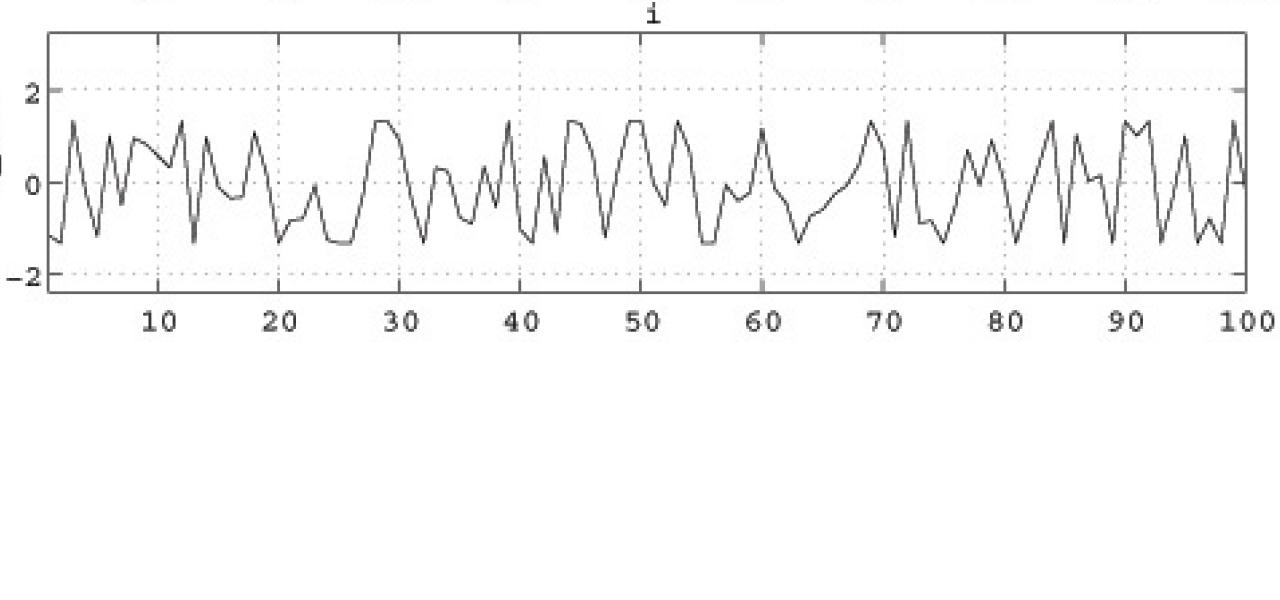
\includegraphics[scale=0.3]{residus.jpg}
    \end{center}

    \begin{solution}
      Le vecteur $b \notin Col(A) $ si et seulement si le nombre de contraintes est strictement supérieur au nombre de variables (en faisant l'hypothèse que les contraintes sont linéairement indépendantes). Pour plus d'explications, voir transparents CM 3.
    \end{solution}

  \item Vrai ou faux? Justifiez vos choix par quelques lignes, un contre-exemple ou un dessin. Soyez assez précis pour convaincre
    que vous ne devinez pas la réponse mais ne fournissez toutefois pas une justification formelle et détaillée.

    \begin{enumerate}

% polyhedron

      \item L'union de deux polyèdres est un polyèdre.

%\item The empty set is a polyhedron.

%extreme points

      \item Tout polyèdre $P$ peut être écrit sous forme géométrique $P=\{ {\bf x} \in {\bf R}^n: \bf A \bf x\geq \bf b\}$.

      \item Tout polyèdre $P$ peut être écrit sous forme standard
        $P=\{ {\bf x} \in {\bf R}^n: \bf A \bf x= \bf b, \bf x \geq 0\}$.


% \item L'ensemble $\{(x,y,z):x^2+y^2+z^2\leq 1\}$ est un polyèdre.

%\item A polyhedron in standard form always has an extreme point.

%\item A non-empty bounded polyhedra has at least one
%non-degenerate vertex.

%\item A point in a polyhedron in standard form can be expressed as
%a convex combination of the polyhedron vertices.

%\item Let $x_0$ and $x_1$ be two vertices of a polyhedron in ${\bf
%R}^n$ and let the polyhedron be defined by $m$ linear
%inequalities. Then here is a path from $x_0$ to $x_1$ along edges
%of the polyhedron that passes through at most $m^m$ edges.

%\item If there exists a vector $\bf q \neq \bf 0$ for which $\bf A
%\bf q=\bf 0$, then the polyhedron $\{\bf x: \bf A \bf x\geq \bf
%b\}$ doesn't have any vertex.

%\item Suppose that the polyhedron $\{{\bf x}: \bf A \bf x\geq \bf
%b\}$  is non-empty and bounded, then $\bf x = \bf 0$ is the only
%vector for which $\bf A \bf x = \bf 0$.

% solutions

      \item L'ensemble des solutions optimales d'un problème d'optimisation linéaire est un polyèdre.

%Consider the set $Q$ of optimal solutions to $\min \{ {\bf c}'
%{\bf x}: {\bf A} {\bf x} \geq {\bf b}, {\bf x} \in {\bf R}^n\}$.
%The set $Q$ is a polyhedron and its extreme points are extreme
%points of the polyhedron $\{{\bf x} \in {\bf R}^n: \bf A \bf x
%\geq \bf b\}$.

%\item A linear optimization problem may have exactly two optimal
%solutions.


%\item At an optimal solution of a linear optimization problem in
%${\bf R}^n$ there are $n$ active constraints.

      \item En toute solution optimale d'un problème d'optimisation linéaire de
        $n$ variables il y a au moins $n$  contraintes actives.


%\item Let $\bf x$ be a basic feasible solution associated with
%some basic matrix. If $\bf x$ is the unique optimal solution, then
%the reduced cost of every nonbasic variable is positive.

% simplex




%\item If a linear optimization problem has an unbounded optimal
%cost, then its dual is infeasible.


%\item If a linear optimization problem is infeasible, then its
%dual has unbounded optimal cost.


%\item L'optimisation linéaire permet de faire une régression linéaire minimisant la norme $||\cdot||_\infty$ des résidus.


    \end{enumerate}

    \begin{solution}
      a) Faux, b) Vrai, c) Faux, d) Vrai, e) Faux
    \end{solution}

\end{enumerate}
